\chapter{Не решённые и только-что решённые}


\setlength{\epigraphwidth}{.80\textwidth}
\epigraph{Мы должны знать --- мы узнаем!
}{--- Давид Гильберт (1862---1943)}

Плохая новость: эта глава может вас сломать.
Но есть и хорошая новость: нерешённая задача не значит, что она неразрешимая.
На самом деле две из нерешённых головоломок моей предыдущей книги были недавно решены.
Первая была особенно известной, и с ней произошло нечто по истине удивительное.

\section*{Ангел и дьявол Конвея}

Ангел летает над бесконечной шахматной доской и время от времени
должен садиться на клетку.
Он может пролететь не более 1000 ходов
короля до очередного приземления.

Пока ангел летит, дьявол, живущий под доской, может уничтожить клетку на свой выбор.

Сможет ли дьявол добиться того, что ангелу некуда будет приземлиться?

\medskip

Поразительно и непостижимо, но эта головоломка, открытая тридцать лет, была внезапно решена
четыре раза
независимо и почти одновременно
людьми из четырёх стран \cite{10, 20, 40, 43}.

Методы были по большей части схожими, и они не опиралась на недавно разработанные новые методы.
На самом деле, все доказательства основывались на наблюдениях, сделанных самим Джоном Конвеем ещё в 70-х.
Четверо решивших были
Андраш Мате, из Университета имени Этвёша Лоранда в Будапеште;
Брайан Боудич, из Университета Саутгемптона;
Оддвар Клостер, из SINTEF ICT в Осло; и Питер Гакс, из Бостонского университета.
Было давно известно, что ангела мощности 1 (который перемещается на один ход короля) можно победить.
Мате и Клостер показали, что ангел мощности 2 выигрывает;
Боудич доказал, что достаточно мощности 4,
а Гакс, что какой-то мощности $p$ достаточно.

Доказательства оказались достаточно простыми, так что Бела Боллобаш, из Кембриджского университета и Университета Мемфиса, смог объяснить их все на восхитительном одночасовом докладе в Университете Иллинойса.
Далее следует выжимка из его доклада и статьи Мате, доказывающей, что ангел мощности 5 выигрывает.

Идея в следующем, если доказать, что ангел выигрывает (в несколько более сильном смысле) против несколько более слабого противника, называемого \emph{добрым дьяволом}, то он сможет выиграть и против изначального (\emph{злого}) дьявола.
Как мы увидим, против доброго дьявола сработает удивительно простая стратегия.

Доброму дьяволу запрещено уничтожать клетку, на которую ангел мог бы прыгнуть ранее;
другими словами, все клетки на расстоянии от $0$ до $p$ от любой клетки посещённой ангелом ранее, доброму дьяволу становатся недоступными.
Легко проверить, что ангел может выиграть в изначальной игре, если, для любого $n$, он может уйти на расстояние $n$.
Теперь мы покажем, что если он может такое проделать с добрым дьяволом, то сможет и со злым.

Предположим, у злого дьявола есть стратегия, удерживающая ангела на расстоянии $n$ от начальной клетки.
Сейчас мы покажем, как добрый дьявол может сделать то же самое.
По данной последовательности ходов ангела, построим \emph{сокращённую} последовательность следующим образом.
Пусть $A_1$ --- самая ранняя клетка посещённая ангелом, с которой он мог бы прыгнуть на последнюю клетку $A_0$.
Удалим все ходы между $A_1$ и $A_0$.
Далее пусть $A_2$ --- самая ранняя клетка посещённая ангелом, с которой он мог бы прыгнуть прямо на $A_1$.
Удалим все ходы между $A_2$ и $A_1$.
Продолжая таким образом, мы получаем укороченную версию $A_k$, $A_{k-1}, \dots, A_1$, $A_0$ исходной последовательности, в которой ангел никогда не прыгает в точку, с которой мог бы перейти ранее.

Теперь заставим доброго дьявола реагировать на данную последовательность ходов так, как это сделал бы злой дьявол в ответ на сокращённую последовательность, с одним изменением --- если требуется съесть недозволенную клетку (или она уже съеденна), то вместо этого дьявол съедает любую допустимую.
Легко показать, что если данная последовательность работает для ангела против доброго дьявола (то есть, он не заставит ангела приземлиться на съеденную клетку), то сокращённая версия этой последовательности срабатывает против злого дьявола.
Таким образом, если он может уйти на расстояние $n$, играя против доброго дьявола, то он сможет сделать то же самое и против злого, и таким образом выиграть.

\begin{figure}[htb!]
\centering
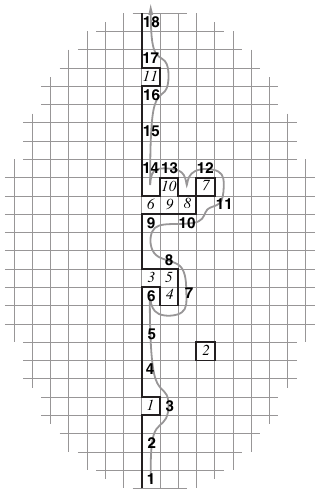
\includegraphics[scale=1]{pics/angel}
\caption{Стена отмечена чёрным, ангел --- жирным шрифтом, добрый дьявол --- курсивом.}
\label{pic:angel}
\end{figure}

Мы свели задачу к убеганию от доброго дьявола, а сделать последнее очень просто,
ангел может даже позволить себе бегать, не прыгая, по несъеденным клеткам.
Он начинает на клетке, нижний левый угол которого находится в начале координат, и представляет себе стену вдоль линии $y = 0$.
Каждый раз, когда добрый дьявол съедает клетку, он возводит стену вокруг этой клетки.
Тем временем, на каждом ходу, ангел бежит в основном на север, держа стену непосредственно слева от себя, пока это можно.
Иногда ангелу придётся бежать на юг, чтобы обойти какой-то участок стены, но мощности $5$ достаточно, чтобы гарантировать, что он продвинется на север по крайней мере на единицу за каждый сделанный шаг.
Отсюда следует, что ангел мощности $5$ может уйти произвольно далеко.
Проделав дополнительную работу можно убедиться, что и мощности $2$ достаточно.
На рис. \ref{pic:angel} показан возможный путь для ангела мощности~$2$.

Стратегия для ангела, описанная выше, конечно же не работает против злого дьявола, который может, например, подготовить ловушку для ангела далеко по оси $y$ --- он заманит наглела в конец полуострова, окружённого морем съеденных клеток, и затем отрежет его от берега.
Хороший дьявол не может этого сделать, ведь ему нельзя уничтожить вход на полуостров после того, как ангел туда прошёл.

К сожалению, то как стратегию убегания от доброго дьявола можно превратить в стратегию против злого, объяснить довольно трудно объяснить, даже при том, что построение выше довольно прямолинейно.
От части это и объясняет, почему головоломка оставалась так долго открытой, подтверждая при этом, что сокращения --- мощный метод решения.

\begin{addedbytheeditors}
\textbf{Редакторам:} Мутный оригинал и мутный перевод. Сам в доказательтве не разбирался, но может кому-то это интересно и этот кто-то всё перепишет?
\end{addedbytheeditors}


\medskip

Следующей головоломке ещё далеко до полного решения,
однако до недавнего времени про неё вовсе ничего не было доказано.

\section*{Затор}

Вершины бесконечной решётки на плоскости выбираются независимо с
фиксированной вероятностью $p\in (0,1)$.
В каждую из выбранных вершин
помещают автомобиль, направленный либо на север, либо на восток, в
каждом случае направление выбирается независимо подкидыванием монеты.

Движение регулируется светофорами, которые включают поочерёдно
«зелёный-восточный» и «зелёный-северный».
При включённом
зелёном-восточном каждый автомобиль, направленный на восток, правая
соседняя вершина от которого не занята, перемещается в эту вершину;
остальные (в том числе заблокированные другим восточным автомобилем)
остаются на месте.

Когда включается зелёный-северный, каждый незаблокированный
автомобиль, направленный на север, перемещается на одну вершину в
северном направлении.

Эксперименты показывают, что если $p$ меньше определённого
критического значения $p_0$, то автомобили постепенно разъедутся
(каждый автомобиль имеет предельную скорость,
равную скорости автомобиля, который никогда не блокируется).
Но когда
$p> p_0$, происходит обратное: автомобили попадают в безнадёжный
затор, то есть каждый автомобиль совершает лишь конечное число переездов
и останавливается навсегда.

Эту модель движения транспорта на перекрёстке двух крупных односторонних улиц представили О. Бихам, А. А. Миддлтон и Д. Левин в 1992 году \cite{6}.
Её странное поведение привлекло много внимания.
%библиографию можно найти по ссылке http://cui.unige.ch/spc/Bibliography/traffic.html.
%недоступная и незархивированя ссылка??? 

\begin{figure}[htb!]
\centering
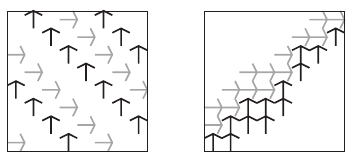
\includegraphics[scale=1]{pics/gridlock}
\caption{Свободное движение слева и затор справа.}
\label{pic:gridlock}
\end{figure}

На рис. \ref{pic:gridlock} изображены конечные части свободной конфигурации и конфигурации с затором, каждая из которых типична для того, что появлялось в экспериментах, проводимых Раисой Де Соуза \cite{15}, ныне преподаватель Университета Калифорнии в Дэвисе.

Весной 2005 года в Исследовательском институте математических наук в Бёркли, Омер Ангел, Эндер Холройд и Джеймс Мартин наконец-то добились прогресса: они доказали, существование фазы затора.
Другими словами, при достаточно высокой плотности машин произойдёт затор, и каждая машина в конечном итоге совершит лишь конечное число переездов.
Доказательство использует теорию перколяций и не будет повторено здесь, но оно весьма изобретательно, и с ним очень стоит ознакомиться \cite{2}.

Конечно же, каждый раз, когда решается одна математическая задача, появляются три новые.
Думаю, что следующие несколько красавиц заслуживают внимания.

\subsection*{Упаковка прямоугольников}

Дан конечный набор точек в квадрате, включающий его нижний левый угол.
Разрешается выбрать набор непересекающихся прямоугольников, лежащих в квадрате, левые нижние вершины которых образуют данный набор точек.
Можно ли выбрать прямоугольники так, чтобы их общая площадь была не меньше половины площади всего квадрата?

\medskip

Эту сбивающую с толку задачу я узнал больше десяти лет назад,
о ней мне сообщил Билл Паллиблэнк (математик и администратор) из IBM, который не помнил, откуда он её узнал.
С тех пор задача всплывала то там, то сям, но мне не удалось найти более ранний источник.
В июне 2004 года она появилась на веб-странице головоломок IBM \cite{ponder-this}, но так и осталась нерешённой.
Я даже не знаю доказательство того, что прямоугольники могут покрыть 1\% площади квадрата.

\begin{figure}[htb!]
\centering
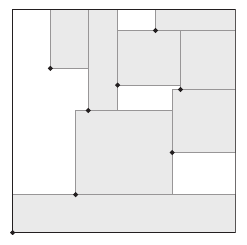
\includegraphics[scale=1]{pics/square}
\caption{Прямоугольники покрывают больше половины площади.}
\label{pic:square}
\end{figure}

На рис. \ref{pic:square} изображена конфигурация точек вместе с подходящим набором прямоугольников.

\subsection*{Произведения и суммы}

Можно ли раскрасить неотрицательные целые числа $\{0,1,2,\dots\}$ конечным числом цветов так, чтобы сумма $x+y$ и произведение $xy$ любых двух целых чисел были разных цветов?

\medskip

Эта задача была предложена Дэвидом Гэлвином, постдоком в Университете Пенсильвании.
Вроде как известен набор из шести чисел такой, что любые два из них являются произведением и суммой некоторой пары чисел, так что для раскраски потребуется по крайней мере шесть цветов.
С другой стороны, известно, что не существует произвольно больших наборов чисел с указанным свойством.

\medskip

Следующая загадка связана с игрой под названием «Давление», придуманной Борисом Алексеевым из Университета Джорджии, в неё играла команда США на недавней математической олимпиаде.

\subsection*{Давление}

Двум игрокам сдают по некоторому числу карт, сначала в открытую (рубашкой вниз),
на каждой карте написано целое число, все числа различны.
В каждом раунде игроки одновременно выкладывают по карте;
более высокая карта сбрасывается, а более низкая передаётся другому игроку.
Проигрывает тот у кого кончились карты.

При увеличении числа сдаваемых карт,
какова предельная вероятность того, что у одного из игроков будет выигрышная стратегия?

\medskip

Борис (как и я) подозревает, что эта вероятность стремится к нулю, но анализ этой простой вариации игры в пьяницу кажется сложным.

\medskip

А вот неожиданная загадка от Стива Хедетниеми из Университета Клемсона:

\subsection*{Покрытие ферзями}

Пусть $f(n)$ --- минимальное число ферзей, которые можно расставить на доске размера $n \times n$ так, чтобы каждая клетка была под ферзём или под боем ферзя.
Верно ли, что $f(n + 1) \geqslant f(n)$ при вех $n$?

\medskip

Есть множество головоломок о расстановке шахматных фигур (обычно ферзей или коней) на доске размером $n \times n$; с ферзями обычно целью является размещение как можно большего количества так, чтобы ни один ферзь не бил другого, но нам нужно наменьшее число ферзей для покрытия всех клеток.
Кажется трудно поверить, что для покрытия меньшего количества клеток вам может понадобиться больше ферзей, однако на большей доске есть больше мест, откуда ферзь может контролировать свои владения, и это трудно исключить!

\medskip

А вот увлекательная, но на самом деле довольно серьёзная головоломка, которая уже многие годы сбивает с толку специалистов по оптимизации.

\subsection*{Встреча}

Двое друзей потеряли друг друга в огромном торговом центре.
На поиск друг-друга в одном магазине у них уходит по 15 минут,
при этом время перемещения от одного магазина к другому ничтожно мало
(торговый центр хорошо организован в виде огромного многоэтажного квадрата).
Они не договорились о месте встречи и не определили заранее, кто будет искать, а кто останется на месте.
Как им следует действовать, чтобы минимизировать ожидаемое время до встречи?

\medskip

Если один из них ищет, а другой ждёт на месте, то в среднем потребуется проверить $n/2$ магазинов, где $n$ --- число магазинов в торговом центре (предполагается, что оно большое).
Однако правила запрещают протокол, нарушающий симметрию, то есть, нельзя например, указывать, что младший будет искать, а старший останется на месте.
Если оба ищут, то в среднем потребуется $n$ шагов, прежде чем они окажутся в одном и том же магазине в одно и то же время и найдут друг-друга.

Эта задача была поставлена в 1976 году (хотя не в этих словах) Стивом Альперном из Лондонской школы экономики.
О ней и некоторых других задачах можно почитать на веб-сайте Ричарда Вебера из Кембриджского университета \cite{weber}.
Вебер и Э. Дж. Андерсон предложили алгоритм, согласно которому каждый друг бросает изогнутую монетку, решая с вероятностью около $0{,}2475$ остаться на месте, проверять магазины в случайном порядке;
и в случае неудачи повторить процесс.
Это приводит к успеху в среднем за $0{,}8289n$ шагов, однако никто не смог доказать то, что это оптимально.

\subsection*{Подкрученный прямоугольник}

Как вы, вероятно, знаете, ленту Мёбиуса можно получить из длинной прямоугольной бумажной ленты,
подклеив на пол оборота её концы.
А какой длины нужна полоса?
Иными словами, какие пропорции прямоугольника из бумаги, наиболее подходящие для создания ленты Мёбиуса, без растяжения или сгибания?

Дмитрий Фукс и Сергей Табачников представляют эту головоломку \cite[Лекция 14]{19} вместе с доказательством того, что необходимо отношение длины к ширине, равное $\pi/2 \sim 1{,}57$, и достаточно отношение $\sqrt{3} \sim 1{,}83$.
Однако точный ответ неизвестен.

\begin{addedbytheeditors}
Задача решена Ричардом Шварцем \cite{schwartz}.
\end{addedbytheeditors}


\subsection*{Автоматы жевательной резинки}

Различные автоматы с жевательной резинкой в местной игровой зоне работают случайным образом, иногда выдавая много жевательных резинок, а иногда вообще ничего не выдавая.
Однако каждый автомат в среднем выдаёт одну жевательную резинку за раз.
Какова максимально возможная вероятность того, все $n$ автоматов за раз выдадут больше чем $n$ жевательных резинок?

\medskip

Эта головоломка (сформулированная в терминах независимых случайных переменных) принадлежит Ури Фейге из Microsoft Research.
Кажется оптимальным заставить каждый автомат выдавать $n + 1$ жевательных резинок с вероятностью $1/(n + 1)$,
а иначе ни одной.
В этом случае мы больше, чем $n$ жевательных резинок если хоть один автомат сработал.
Это происходит с вероятностью
\[1-(1-\tfrac1{n+1})^{n+1},\]
которая подходит к $1 - 1/e \sim 63\%$, при больших $n$.
Пока никто не придумал ничего лушего.
Сам Фейге доказал, что вероятность получить более чем $n$ жевательных резинок не может превысить $12/13$.
Но ведь не может это быть так уж сложно.

\subsection*{Круги на плоскости}

Дано множество открытых единичных кругов, которое тысячекратно покрывает плоскость;
то есть, каждая точка $\mathbb{R}^2$ покрывается как минимум тысячью кругами.
Докажите, что круги можно раскрасить в красный и синий цвета так,
чтобы красные и синие круги по отдельности покрывали всю плоскость.

\medskip

Янош Пах из Нью-Йоркского университета является создателем (и экспертом по) этой замечательной открытой задаче.
В своей статье \cite{46} он доказал, что для любого симметричного многоугольника $P$ и любого положительного целого числа $r$ существует число $k$, такое что любое $k$-кратное покрытие плоскости параллельными переносами $P$ можно разбить на $r$ покрытий.
Но если многоугольник заменить на круг, то неизвестно есть ли такое $k$, даже для $r = 2$.

Я считаю, что $k = 4$ должно хватить.
А вы, что скажите?
